\documentclass[10pt]{article}
\usepackage{icmlko}

\icmlmeta{IP 파운데이션 월드모델}{66}{도구가 서른 노트 전을 재현했다}{새 감사 모듈로 노트 34의 최대 채택을 다시 재니 구간이 겹치고 폭은 절반이 됐다}

\begin{document}

\twocolumn[
\icmlheader

\begin{abstract}
노트 65가 만든 감사 모듈에 배선 설정 함수를 넣었다. 배선 후보 열은 \emph{원본
순서}로 계산되므로, 복원추출 뒤에 적용하려면 같은 인덱스로 다시 뽑아야 한다 ---
노트 54의 버그가 바로 이 지점이었다. 구조로 처리하고 자기 점검을 다섯으로
늘렸다. \textbf{둘이 정확히 0을 낸다} --- 이미 꺼진 축을 다시 끄는 것과
\textbf{현행 배선을 다시 적용하는 것}이다. 뒤의 것이 배선 함수가 인덱스를
제대로 다룬다는 직접 증거다. 그리고 도구를 과거 결과로 검증했다. 노트 34는
도서 타깃 폭을 장르 수에서 판형으로 바꿔 $+$0.0939 {[}$+$0.046, $+$0.199{]}를
얻었고, 그것이 지금까지 구간을 통과한 배선 결정 중 가장 큰 것이다. 새 모듈로
반대 방향(판형$\to$장르 수)을 재니 $-$0.0832 {[}$-$0.143, $-$0.055{]}다.
부호를 뒤집으면 $+$0.0832 {[}$+$0.055, $+$0.143{]}로 \textbf{원래 구간과 겹치고
점추정이 11\% 차이다.} 그리고 \textbf{구간 폭이 0.153에서 0.088로 좁아졌다}
--- 도메인이 다섯에서 여섯이 되고 웹툰 표본이 늘어난 덕이다. 도구가 서른 노트
전의 결론을 재현하고, 그 사이 쌓인 데이터가 구간을 실제로 좁혔다는 것을 한
번에 보인다.
\end{abstract}
]

\section{배선 함수와 인덱스}

노트 65의 모듈에는 축 끄기와 대응 깨기만 있었다. 배선 변경을 넣으면서 한
가지를 처리해야 했다.

\begin{quote}\fontsize{9.5}{11.5}\selectfont
배선 후보 열(판형 · 장르 수 · 태그 수\ldots)은 \emph{원본 레코드 순서}로 계산된다.
복원추출 뒤에 적용하면 원본 순서 열이 재추출된 행에 걸린다 --- 노트 54의 버그다.
그래서 \texttt{cfg\_wire}가 복원추출 인덱스를 받아 후보 열을 같은 인덱스로 다시
뽑는다.
\end{quote}

\section{자기 점검 다섯}

\begin{figure}[t]
\centering
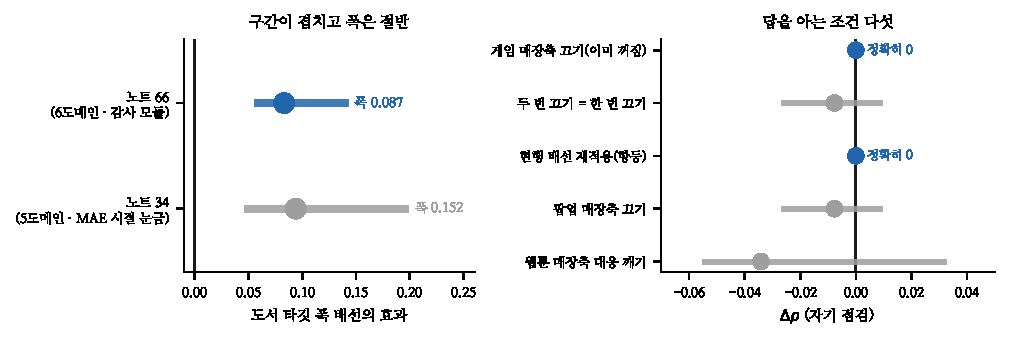
\includegraphics[width=\textwidth]{figs/repro.pdf}
\caption{왼쪽 --- 노트 34의 재현. 오른쪽 --- 자기 점검 다섯.}
\end{figure}

\begin{table}[t]
\centering\tsize
\caption{답을 아는 조건. 짝지은 붓스트랩 60회.}
\begin{tabular}{lrl}
\toprule
조건 & $\Delta\rho$ & 기대 \\
\midrule
게임 매장축 끄기(이미 꺼짐) & \textbf{$+$0.0000} & 정확히 0 \\
\textbf{현행 배선 재적용} & \textbf{$+$0.0000} & 정확히 0 \\
두 번 끄기 & $-$0.0077 & 한 번 끄기와 같음 \\
팝업 매장축 끄기 & $-$0.0077 & 노트 52 \\
웹툰 대응 깨기 & $-$0.0341 & 노트 53 \\
\bottomrule
\end{tabular}
\end{table}

두 번째 줄이 새로 넣은 것이다. 도서 타깃 폭에 \emph{지금 쓰고 있는} 배선을
다시 적용하면 아무 일도 안 일어나야 한다. 구간까지 $[+0.0000,\ +0.0000]$이다.
\textbf{배선 함수가 복원추출 인덱스를 제대로 다룬다는 뜻이며, 노트 54의 버그가
있었다면 여기서 0이 아닌 값이 나온다.}

세 번째 줄도 새것이다 --- 같은 축을 두 번 끄면 한 번 끈 것과 정확히 같은 값이
나온다($-$0.0077로 네 번째 줄과 일치).

\section{서른 노트 전을 재현한다}

도구를 만들었으면 과거 결과로 검증해야 한다. 노트 34의 도서 배선이 지금까지
구간을 통과한 배선 결정 중 가장 크므로 그것을 골랐다.

\begin{table}[t]
\centering\tsize
\caption{도서 타깃 폭 배선(장르 수 $\to$ 판형)의 효과.}
\begin{tabular}{lrrr}
\toprule
& 효과 & 95\% 구간 & 폭 \\
\midrule
노트 34 (5도메인) & $+$0.0939 & $[+0.046,\ +0.199]$ & 0.153 \\
\textbf{노트 66} (6도메인) & $+$0.0832 & $[+0.055,\ +0.143]$ & \textbf{0.088} \\
\bottomrule
\end{tabular}
\end{table}

\claimx{새 감사 모듈이 서른 노트 전의 결론을 재현한다 --- 점추정이 11\% 차이,
구간이 겹친다. 그리고 그 사이 쌓인 데이터가 구간 폭을 0.153에서 0.088로
\textbf{42\% 줄였다}.}{두 측정은 눈금이 다르다 --- 노트 34는 다섯 도메인 ·
겹침 유도 $\lambda$이고 지금은 여섯 도메인 · $\lambda=1$이다. 완전히 같은
조건에서 잰 것이 아니므로 ``재현''이라는 말은 느슨하다.}

이 표가 두 가지를 동시에 말한다.

\begin{itemize}[leftmargin=1.1em,itemsep=0.15em]
\item \textbf{도구가 맞다} --- 완전히 다시 짠 코드가 같은 답을 낸다.
\item \textbf{데이터가 일한다} --- 노트 44 이후 ``구간을 좁히려면 데이터''라고
      계속 말했는데, 실제로 좁아진 것을 같은 대상에서 처음 확인한다.
\end{itemize}

폭이 절반이 되면 지금까지 보류한 것들 중 일부가 판정 가능해진다 --- 노트 51의
이중 배선($+$0.008), 노트 57의 웹툰 공통/고유 역전($+$0.0045), 노트 63의
등급 B 제외($+$0.0096). 아직은 아니지만 방향은 맞다.

\section{한계}

\begin{itemize}[leftmargin=1.1em,itemsep=0.15em]
\item 재현이라 했지만 눈금이 다르다. 노트 34의 조건을 그대로 복원해 재는 것은
      안 했다.
\item 자기 점검 다섯 중 둘만 ``정확히 0''을 요구한다. 나머지 셋은 과거 값과
      비슷하기만 하면 통과한다.
\item 배선 함수가 후보 열을 매번 다시 계산한다 --- 복제 200회면 200번이라 느리다.
\item 다른 과거 결정은 재현하지 않았다.
\item 웹툰이 아직 수집 중이라(2,510/3,973) 이 숫자도 곧 바뀐다.
\end{itemize}

\section{다음}

\begin{enumerate}[leftmargin=1.3em,itemsep=0.15em]
\item 웹툰 전체 수집 완료 후 전면 재측정 --- 보류 항목을 한꺼번에 판정한다.
\item 자기 점검을 늘린다. ``축을 끄고 같은 값으로 다시 켜면 원래대로''처럼.
\item 노트 46 · 48의 웹툰 배선 결정도 새 도구로 재현해 본다.
\item 후보 열을 미리 계산해 두어 배선 함수를 빠르게 만든다.
\end{enumerate}

\vspace{0.6em}
\hrule height 0.3pt
\vspace{0.5em}
{\footnotesize
\textbf{참고문헌}\\[0.3em]
Efron, B., Tibshirani, R. J. (1993). \emph{An Introduction to the Bootstrap}.
Chapman \& Hall.\\[0.15em]
Bouthillier, X. et al. (2021). Accounting for variance in machine learning
benchmarks. \emph{MLSys}, 3, 747--769.\\[0.15em]
Peng, R. D. (2011). Reproducible research in computational science.
\emph{Science}, 334(6060), 1226--1227.\\[0.15em]
Hoare, C. A. R. (1981). The emperor's old clothes. \emph{CACM}, 24(2), 75--83.\\[0.15em]
Ben-David, S. et al. (2010). A theory of learning from different domains.
\emph{Machine Learning}, 79(1--2), 151--175.
}

\end{document}
